\documentclass[12pt]{article}

\usepackage[T1]{fontenc}
\usepackage[utf8]{inputenc}
\usepackage{lmodern}
\usepackage{amsmath,amssymb,bm}
\usepackage{graphicx}
\usepackage{booktabs}
\usepackage{tabularx}
\usepackage{tikz}
\usepackage[labelfont=bf,labelsep=period]{caption}
\usepackage{titlesec}
\usepackage[a4paper,top=2cm,bottom=2cm,left=3cm,right=1.5cm]{geometry}
\usepackage[hidelinks]{hyperref}
\usetikzlibrary{arrows.meta,positioning,calc,shapes.geometric}

\setlength{\parindent}{1.25em}
\setlength{\parskip}{0pt}
\renewcommand{\figurename}{Fig.}
\renewcommand{\tablename}{Table}
\renewcommand{\refname}{REFERENCES}
\titleformat{\section}{\normalfont\normalsize\bfseries\centering}{}{0pt}{\MakeUppercase}
\titlespacing*{\section}{0pt}{2.0ex plus 0.5ex minus 0.2ex}{1.0ex plus 0.2ex}
\titleformat{\subsection}{\normalfont\normalsize\bfseries}{}{0pt}{}
\titlespacing*{\subsection}{0pt}{1.6ex plus 0.4ex minus 0.2ex}{0.8ex plus 0.2ex}

\tikzset{
refgbox/.style={draw, rounded corners=2pt, align=center, inner sep=5pt, minimum height=0.9cm, font=\small},
refgarrow/.style={-{Latex[length=2.2mm]}, thick},
regimebox/.style={draw, rounded corners=2pt, align=center, inner sep=5pt, minimum width=3.2cm, minimum height=1.05cm, font=\small},
markerbox/.style={draw, rounded corners=2pt, align=center, inner sep=4pt, font=\small}
}

\begin{document}

\begin{center}
\vspace*{1.15cm}
{\large\bfseries Refractive Gravity: A Phase-Field Theory\par}
\vspace{1.65em}
George Lotishvili\textsuperscript{a,*} (\href{https://orcid.org/0009-0009-6788-713X}{ORCID 0009-0009-6788-713X})\\
\vspace{1.45em}
\textsuperscript{a}\textit{East European University, Tbilisi, Georgia}\\
\textit{Independent researcher}\\
\vspace{1.15em}
\textsuperscript{*}\textit{e-mail:} \href{mailto:g_lotishvili@eeu.edu.ge}{\texttt{g\_lotishvili@eeu.edu.ge}}
\end{center}

\vspace{1.1em}
\noindent\textbf{Abstract---}
Refractive Gravity (RefG) is a phase-spatial effective field theory built on a metric theory of gravity. Its geometric core is the Einstein--Hilbert term, while the new sector consists of one phase scalar $\Phi$, three spatial medium scalars $\phi^A$, and their couplings. The paper focuses on the minimal self-contained core: the action, active stress, refractive source, weak-field limit, cosmological balance, and observational consistency conditions.

The physical mechanism is the following. Matter creates a phase-pressure deficit in the base medium; the active stress obtained from the action is collected, in the weak static regime, into the variable $h_{\rm eff}$; the minimal metric coupling of matter and the static optical limit define the refractive index $n_{\rm eff}=\exp(h_{\rm eff})$; and the acceleration of test matter is determined by the gradient of this index. In the local spherical channel the Bernoulli response gives Newton's law, while in the coherent vortical channel the same source equation describes the deep-MOND limit and the baryonic Tully--Fisher relation (BTFR).

The mathematical results obtained in the paper are as follows. The quadratic Bernoulli pressure and the linear Tolman--Oppenheimer--Volkoff (TOV) source are unified through the response density $\Pi_B'$; the branch $C_6=Y+2I_1-I_3=6$ provides a background $\Lambda$CDM-type balance with the normalization $\rho_0$; the weak-field Solar-System branch preserves $\gamma=\beta=1$, $\alpha_i=0$, and the GR-compatible coefficient $q_{\rm 2PN}=7/4$; in the tensor sector the gravitational-wave speed is equal to the speed of light, $c_g=c$; and the extra linear sources vanish for the cosmic microwave background (CMB) test with identical input conditions. In the leading phase-spherical strong-field branch, the vacuum phase equation and the biconformal operational map give an exponential exterior. The geodesic analysis of this exterior gives $r_{\rm ph}=r_s$, $b_c=e r_s$, $r_{\rm ISCO}=\varphi^2 r_s$, and $f_{\rm ISCO}=0.931\,f_{\rm ISCO}^{\rm GR}$. This is the central falsifiable static marker of the paper: the static shadow scale shifts by $+4.63\%$ relative to the Schwarzschild value in GR.

The strong-field phase branch is distinct from the weak physical Solar-System exterior: near the Sun, diffuse medium stress remains in the 2PN balance and gives $q_{\rm 2PN}=7/4$; outside an ultradense compact source, the exterior phase vacuum enters the exponential branch. The full data layer includes the $H(z)/w(z)$ channel, SPARC/RAR and cluster comparison, the active CMB problem without particle dark matter, additional gravitational-wave polarizations, and EHT/ngEHT/BHEX tests of the rotating strong-field sector.

\noindent\textbf{Keywords:} refractive gravity; modified gravity; effective field theory; MOND; cosmology; compact objects

\section{Introduction}

General relativity describes gravity in the language of metric geometry. This formalism works with high precision in the Solar System, in binary pulsars, in gravitational waves, and in the geometric sector of the standard cosmological model. Refractive Gravity (RefG) preserves this core: the metric still determines the light cone, the minimal coupling of matter, and geodesic motion.

RefG adds a phase-spatial medium to this geometric core. The local state of the medium is described in the action through invariants, and its variation produces an additional stress tensor. The weak-field branch of this stress appears to an external observer as a refractive profile. The name ``Refractive Gravity'' refers to the physical source mechanism: the metric response follows from a phase-pressure deficit that acts refractively on wave-like bodies and on light.

The difference from the standard approach appears at two levels. At the geometric level, RefG preserves the strict structure of a metric theory: particles are minimally coupled to the metric, and free bodies move along geodesics. In the weak field, writing the metric profile through an optical index is a standard representation. The new content of RefG lies in the source mechanism: the active stress obtained from the action of the phase-spatial medium enters the Bianchi/TOV identity; this identity determines $h_{\rm eff}$; and the static optical limit gives the index $n_{\rm eff}=\exp(h_{\rm eff})$. The same source-index chain forms the Newtonian profile near a localized source and the MOND/BTFR limit in the coherent galactic channel.

On the literature map, RefG touches several established lines: MOND/TeVeS for galactic phenomenology \cite{Milgrom1983,Bekenstein2004}, emergent gravity for the connection between the acceleration scale and cosmology \cite{Verlinde2017}, mimetic gravity for a scalar representation of an additional gravitational component \cite{ChamseddineMukhanov2013}, solid/framid EFT for medium-like spatial fields \cite{Endlich2013,Nicolis2015}, and the exponential geometrical class used in the strong spherical branch \cite{Boonserm2018}. The distinctive part of RefG is the single source-index chain: active stress, refractive index, the weak-field Newton and MOND limits, cosmological balance, and the phase-spherical strong-field markers.

The present paper focuses on the sectors that form a self-contained formal chain. Full comparison with data, exact strong-field solutions, and particle microphysics are treated as subsequent theoretical layers built on this core.

The complete physical picture of the theory includes particles, quantum regimes, strong fields, galactic morphology, and cosmological dynamics. This paper presents the main axis that directly expresses the gravitational mechanism: the refractive source, its Newtonian limit, the galactic weak-field limit, and the required consistency conditions with observational data.

The structural logic of the paper is the following. A localized oscillon in the base medium leaves a phase-pressure tail; this tail generates active stress; in the weak-field limit the active stress is collected into the variable $h_{\rm eff}$; $h_{\rm eff}$ is physically interpreted as the refractive index $n_{\rm eff}$, whose gradient determines the motion of an object. Near a localized source this mechanism gives the Newtonian profile, in the coherent galactic regime it gives the MOND/BTFR limit, and in cosmological averaging it gives a background balance.

\begin{figure}[t]
\centering
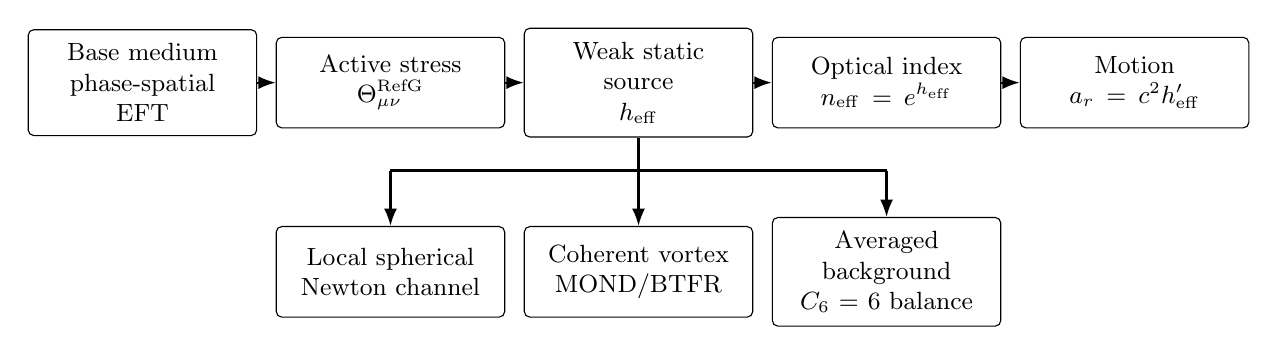
\begin{tikzpicture}[x=3.15cm,y=1.55cm]
\tikzset{
figbox/.style={refgbox, text width=2.55cm, minimum height=1.15cm}
}
\node[figbox] (medium) at (0,0) {Base medium\\phase-spatial\\EFT};
\node[figbox] (stress) at (1,0) {Active stress\\$\Theta^{\rm RefG}_{\mu\nu}$\\{}};
\node[figbox] (source) at (2,0) {Weak static\\source\\$h_{\rm eff}$};
\node[figbox] (index) at (3,0) {Optical index\\$n_{\rm eff}=e^{h_{\rm eff}}$\\{}};
\node[figbox] (motion) at (4,0) {Motion\\$a_r=c^2h_{\rm eff}'$\\{}};

\node[figbox] (newton) at (1,-1.55) {Local spherical\\Newton channel\\{}};
\node[figbox] (mond) at (2,-1.55) {Coherent vortex\\MOND/BTFR\\{}};
\node[figbox] (cosmo) at (3,-1.55) {Averaged\\background\\$C_6=6$ balance};

\draw[refgarrow] (medium) -- (stress);
\draw[refgarrow] (stress) -- (source);
\draw[refgarrow] (source) -- (index);
\draw[refgarrow] (index) -- (motion);

\coordinate (bus) at (2,-0.72);
\coordinate (busleft) at (1,-0.72);
\coordinate (busright) at (3,-0.72);
\draw[thick] (source.south) -- (bus);
\draw[thick] (busleft) -- (busright);
\draw[refgarrow] (busleft) -- (newton.north);
\draw[refgarrow] (bus) -- (mond.north);
\draw[refgarrow] (busright) -- (cosmo.north);
\end{tikzpicture}
\caption{Core source-index chain of RefG. The active stress generated by the phase-spatial medium determines $h_{\rm eff}$; the static optical limit reads this profile as $n_{\rm eff}$; the gradient of the index gives the observed acceleration.}
\label{fig:source-index}
\end{figure}

\section{The Base Medium and the Physical Picture}

The physical conception of RefG is based on a base medium. It is the universal substrate from whose structural elements measurable distance, time, mass, and waveforms are built. Observable physics appears when the base medium branches into phase, spatial, and resonant regimes. Accordingly, space, time, and mass are not independent containers in this theory; they are operational consequences of differentiated regimes of the base medium.

In this paper the base medium and the normalized background are initial operational structures. The paper tests how this structure is written in an effective field theory (EFT) action and how it gives the gravitational source-index chain. The microphysical origin of the base medium and the full oscillon construction belong to a separate theoretical layer.

The terms used in this paper have the following meaning. The base medium is the operational substrate whose regimes form distance, time, and mass. An oscillon is a localized source of phase energy: its far field creates an asymptotic refractive charge. Active stress is the tensor $\Theta^{\rm RefG}$ obtained by varying the action and entering the Bianchi/TOV balance. The variable $h_{\rm eff}$ is the phase lag collected in the weak static limit, while $n_{\rm eff}=\exp(h_{\rm eff})$ is its optical index. The biconformal map is the operational map that links the temporal and spatial metric factors through one phase profile.

In this formalism, matter is treated as a locally closed oscillon state. An oscillon creates a stable trace, or tail, in the medium, and this tail generates a phase-pressure deficit. This deficit determines the effective refractive index. The evolution of another wave-like object takes place in the gradient of this index, which appears macroscopically as gravitational attraction.

A localized source creates a spatially varying phase-pressure deficit in the base medium. On local scales, the observable quantity is the gradient of this deficit, which is read as refractive acceleration. In cosmological averaging, the asymptotic remnants of many sources form a homogeneous background level; a homogeneous background has no local direction and appears as a background balance.

In this picture, physical scales are sharply separated. Near an isolated source, the trace forms a local gravitational profile. On galactic scales, a coherent vortical structure converts the same phase-pressure deficit into an anisotropic MOND-type channel. On cosmological scales, the asymptotic remnant of all source traces forms a homogeneous background, which appears as a global balance and as a recalibration of standards between cosmological epochs.

The local invisibility of the background follows from the fact that measuring devices, such as rods, clocks, and atoms, are formed from the same phase-pressure regime that they measure. A homogeneous global displacement of the medium cancels out of local dimensionless ratios. The observable quantities are a spatial gradient, a phase lag, and the accumulated difference between cosmological epochs. Thus local physical ratios remain stable, while external metric and refractive parameters may evolve.

The fundamental frequency $\nu_0$ of the base substrate is used in this paper as a parameter of the microscopic structural level. Its temporal nature is not determined directly here: macroscopic clocks are themselves formed from operational regimes of the base medium, so the exact translation of $\nu_0$ into laboratory time is a separate problem. Since the microscopic base level affects observable physics, connecting its temporal character to operational time standards belongs to future work.

\section{Fields, Invariants, and the Action}

The question addressed in this section is the following: what is the minimal covariant apparatus by which the phase and spatial response of the base medium can be described through an action principle?

Following the standard logic of effective field theory, one first chooses the fields and then builds coordinate-invariant combinations from them. In RefG, one field describes the phase-time channel, while three fields describe the deformation of the spatial medium. The resulting action integrates temporal excitation, spatial density, shear response, solid-like response, and their mutual coupling.

Their physical interpretation is as follows. The scalar $\Phi$ describes the phase-time component, namely how a composite process propagates between the structural nodes of the base medium. The fields $\phi^A$ describe the spatial, solid-like component, namely how operational distance and medium deformation are defined. Accordingly, the invariants $Y$, $I_1$, $I_2$, and $I_3$ form a minimal covariant basis for phase, spatial density, shear deformation, and volume response.

The metric signature is $(+---)$. The phase scalar is $\Phi$, and the spatial medium fields are $\phi^A$, where $A=1,2,3$. The fundamental invariants are defined by
\begin{align}
Y &= g^{\mu\nu}\partial_\mu\Phi\,\partial_\nu\Phi, \\
B^{AB} &= -g^{\mu\nu}\partial_\mu\phi^A\,\partial_\nu\phi^B, \\
I_1 &= \operatorname{Tr} B, \\
I_2 &= \frac{I_1^2-\operatorname{Tr}(B^2)}{2}, \\
I_3 &= \det B .
\end{align}

The minimal refractive Lagrangian is written as a polynomial in these invariants:
\begin{equation}
F_{\rm min}
= c_Y Y+c_{Y2}Y^2+c_{I1}I_1+c_{I1sq}I_1^2+c_{I2}I_2+c_{I3}I_3+c_{YI1}YI_1 .
\end{equation}

The full action functional takes the form
\begin{equation}
S=\int d^4x\,\sqrt{-g}
\left[
\frac{M_{\rm Pl}^2}{2}R+M_*^4F(Y,I_1,I_2,I_3)
\right]
 + S_{\rm matter}[g,\psi] .
\end{equation}

This formulation sharply separates the minimal dynamical core from the branch-fixing additions. The function $F_{\rm min}$ is the minimal low-energy polynomial basis in the invariants $Y$, $I_1$, $I_2$, and $I_3$: it contains the phase term, the spatial-density term, the shear/volume response, and the $YI_1$ coupling. Higher-order operators form the EFT layer built on this core. The conditions $C_6=6$ and $Z$ are then used to select the background and stability channel in which cosmological balance, local stability, and Solar-System compatibility are tested simultaneously.

The phase sector of the theory maps directly into the minimal Horndeski formalism. With the convention used in the present paper, $Y=-2X$, and therefore
\begin{align}
G_2(X) &= -2c_YX+4c_{Y2}X^2, \\
G_3 &= 0, \\
G_4 &= \frac{M_{\rm Pl}^2}{2}, \\
G_5 &= 0 .
\end{align}

In this minimal model, the excess tensor-mode propagation speed vanishes. For tensor gravitational waves this gives the strict result
\begin{equation}
c_g=c .
\end{equation}

The paper uses the active-medium convention for the energy-momentum tensor. To separate it by sign from the standard matter stress tensor, it is denoted by $\Theta^{\rm RefG}$:
\begin{equation}
\Theta^{\rm RefG}_{\mu\nu}
=2\frac{\partial \mathcal L_{\rm RefG}}{\partial g^{\mu\nu}}
-g_{\mu\nu}\mathcal L_{\rm RefG} .
\end{equation}

The variation with respect to off-diagonal symmetric variables is computed with the appropriate factors following from the symmetry $g^{\mu\nu}=g^{\nu\mu}$. With this convention, the quantities $\rho$, $p_{\rm rad}$, and $p_{\rm tan}$ are active-medium sources that enter, with the same sign convention, the FLRW balance, the Solar-System stress closure, and the projected Bianchi and Tolman--Oppenheimer--Volkoff equations of RefG. The matter sector, in turn, preserves the standard minimal coupling to the metric through the action $S_{\rm matter}[g,\psi]$.

\section{The Refractive Source and Newton's Law}

The question in this section is how the phase-pressure deficit generated by matter is converted into the observable acceleration described by Newton's law.

In the standard formalism, the source curves spacetime and a test body moves along a metric geodesic. In the optical language of the weak field, the same profile can be written as a refractive index. RefG turns this optical language into a source theory: matter is a localized oscillon structure; the oscillon creates a phase-pressure deficit in the base medium; the active stress obtained by varying the action is collected in the Bianchi/TOV balance; this balance determines $h_{\rm eff}$; the static optical limit gives $n_{\rm eff}=\exp(h_{\rm eff})$; and the gradient of the index bends the phase of a wave-like body. To a macroscopic observer this process appears as gravitational acceleration.

The present analysis is based on the following minimal assumptions: the static weak-field limit is considered; matter preserves minimal coupling to the metric; the exterior response is described by a single refractive variable; and the anisotropic component vanishes in the local spherical channel. Under these assumptions the formal apparatus leads directly to the working source equation.

For a static weak field, the metric response is written through one refractive variable. A prime denotes differentiation with respect to the radius, $d/dr$:
\begin{align}
g_{tt} &= \exp(-2h_{\rm eff}), \\
n_{\rm eff} &= \exp(h_{\rm eff}) .
\end{align}

On the chosen weak biconformal branch, $n_{\rm eff}$ is the refractive index of the common phase delay. The temporal and spatial metric factors are tightly linked,
\begin{equation}
AB=1+O(U^2),
\end{equation}
so the same $h_{\rm eff}$ controls both the effective potential of slow test matter and the static eikonal optical limit. On this branch, $h_{\rm eff}$ physically expresses the common phase delay, while $n_{\rm eff}$ is its refractive index.

Minimal metric coupling of matter gives
\begin{align}
\frac{V_{\rm eff}}{m} &= -c^2h_{\rm eff}, \\
a_r &= c^2\frac{d\log n_{\rm eff}}{dr}
     = c^2 h_{\rm eff}' .
\end{align}

Thus gravitational acceleration is equivalent to the gradient of the refractive index. The gravitational source, in turn, is produced not by an abstract external force, but by the spatial part of the energy-momentum tensor obtained from the action. For a spherical deformation, the difference between tangential and radial pressures defines the anisotropy,
\begin{equation}
\Delta_p=p_{\rm tan}-p_{\rm rad}.
\end{equation}

The weak-field TOV/Bianchi source is a radial stress balance that includes the radial pressure gradient and the tangential-radial anisotropy term:
\begin{align}
p_{\rm rad}' + \rho_{\rm eff}\Phi_N' - \frac{2\Delta_p}{r} &= 0, \\
\Phi_N &= -c^2h_{\rm eff}.
\end{align}

Here $\rho_{\rm eff}$ is the effective response density that connects the radial source to the gradient of the Newtonian potential. In the weak local limit it plays the role of inertial, or passive, density. In the spherical Bernoulli channel the pressure deficit is
\begin{equation}
\Pi_B=\frac{\exp(-2h_{\rm eff})(h_{\rm eff}')^2}{8\pi G},
\end{equation}
and the response density entering the TOV source is
\begin{equation}
\rho_B=\frac{\Pi_B'}{c^2h_{\rm eff}'}
=\frac{\exp(-2h_{\rm eff})\left(h_{\rm eff}''-(h_{\rm eff}')^2\right)}
{4\pi Gc^2},
\end{equation}
while in the vortical channel it is the coherent state of the medium, $\rho_{\rm eff}$.

The basic working equation for the source of refractive gravity then follows:
\begin{equation}
h_{\rm eff}'=\frac{p_{\rm rad}'-2\Delta_p/r}{c^2\rho_{\rm eff}} .
\end{equation}

The chain $\Pi_B'\to h_{\rm eff}\to n_{\rm eff}$ is a differential/integral bridge in the weak static limit. The radial source of active stress determines the profile $h_{\rm eff}$, and the static optical limit reads this profile as $n_{\rm eff}=\exp(h_{\rm eff})$. In the weak nonrelativistic limit, $\rho_{\rm eff}$ is read as an effective combination of inertial density and radial pressure response. In this section, $G$ is the normalization of the asymptotic charge.

In the local spherical channel the anisotropy vanishes, $\Delta_p=0$, and the Bernoulli response is active. Outside a compact object the source flux is conserved as an asymptotic charge, which gives the exterior $1/r$ profile. The first-order static spherical analysis selects the biconformal branch $AB=1+O(U^2)$, while the Bernoulli deficit supplies the source of this profile. The normalization of the asymptotic charge fixes
\begin{align}
r_s &= \frac{2GM}{c^2}, \\
h_{\rm eff} &= \frac{GM}{c^2r}, \\
\Phi_N &= -\frac{GM}{r}, \\
a &= -\frac{GM}{r^2}.
\end{align}

Thus, in the weak spherical channel, Newton's law is obtained from the refractive-source mechanism. In this core, Newton's constant is tied to the normalization of the asymptotic gravitational charge; its microscopic origin belongs to a deeper working layer of the theory.

The core result of this section is the weak, static, spherically normalized source-index chain: active stress is collected into $h_{\rm eff}$, $h_{\rm eff}$ determines $n_{\rm eff}$, and the gradient of this index gives the Newtonian acceleration. Fully nonspherical disk or cluster PDE solutions are applications of this core and belong to a separate data layer.

The physical interpretation of the result is the following. An oscillon is a closed wave structure of the base medium. Near a massive source, phase propagation is nonuniform: the speed is reduced on one side, and the wave form of the body bends toward the phase delay. Light bending follows the same principle: a gravitational lens is directly the refractive profile of the base medium.

The Bernoulli pressure function is quadratic, while the TOV source enters through the radial derivative. The TOV equation contains the combination $p_{\rm rad}'-2\Delta_p/r$; in the Bernoulli channel this quantity is equivalent to $\Pi_B'$, the radial derivative of the pressure function. Thus the quadratic state function and the linear radial source are tied into one physical chain: the Bernoulli form enters the TOV equation through its derivative and through the anisotropic component that fixes the direction and magnitude of the refractive force.

\section{The Spherical MOND Limit}

In the galactic limit the main question is what causes the effective law of gravity to change at weak accelerations in such a way that rotation velocities obey the baryonic Tully--Fisher relation (BTFR).

In the standard phenomenological formulation of MOND, this regularity is described by an interpolation function and by the acceleration scale $a_0$ \cite{Milgrom1983}. A classical relativistic theoretical context for MOND is TeVeS \cite{Bekenstein2004}. In RefG, the galactic regime goes beyond the spherical Bernoulli tail of an isolated source and includes a large-scale coherent vortical structure of the base medium. This structure produces an anisotropic refractive load which, in the weak-acceleration limit, converts the Newtonian $1/r^2$ profile into the deep-MOND $1/r$ profile.

The logical connection between the concepts is as follows. The baryonic mass determines the asymptotic gravitational charge; phase coherence sets the scale $a_0$; vortical anisotropy creates the source $\Delta_p$; and $\Delta_p$ is integrated into the same refractive source from which Newton's law was obtained in the previous section.

The present section is based on a spherical, weak, and coherent galactic limit. In this limit the working chain of RefG closes through four links: the phase-coherence boundary sets the natural length of the galactic regime; a two-channel vortical closure connects the baryonic Newtonian source to the vortical refractive response; this closure algebraically gives the transition law $\mu(x)=x/(1+x)$; and in the deep limit the same chain gives the MOND profile and the BTFR. The factor $2\pi$ used in this section is the normalization of a full phase cycle. With this normalization, the MOND/BTFR algebra is fixed; the full vortical action is the next layer that determines how this normalization is selected by the dynamics itself.

In the coherent galactic regime, the vortical load plays the dominant role. In this regime the radial derivative of the Bernoulli pressure weakens, while the anisotropic pressure plateau creates an additional refractive source. The plateau normalization is set by the asymptotic mass $M$, the common response density, and the coherence acceleration $a_0$:
\begin{equation}
\Delta_p=\frac{\rho_{\rm eff}}{2}\sqrt{GMa_0}.
\end{equation}
It follows that
\begin{align}
g_{\rm deep} &= \frac{\sqrt{GMa_0}}{r}, \\
v^4 &= GMa_0 .
\end{align}

With this working normalization, the coherent phase length and the acceleration scale are related by
\begin{align}
\lambda_{H0} &= \frac{2\pi c}{H_0}, \\
a_0 &= \frac{c^2}{\lambda_{H0}}
     = \frac{cH_0}{2\pi}.
\end{align}

The factor $2\pi$ denotes the normalization of the phase cycle. With this normalization, the baryonic channel, the vortical refractive channel, and the total acceleration form one algebraic system. In RefG, the cosmological phase scale enters directly into the MOND transition law.

The working basis of the transition law is a two-channel closure: the baryonic Newtonian channel and the vortical refractive channel combine into one total acceleration. Let $g_N$ denote the baryonic Newtonian channel, $g_v$ the vortical refractive channel, and $g=g_N+g_v$ the total acceleration. A minimal variational form of this closure can be written through the effective load potential
\begin{equation}
W(g_v;g_N)=\frac{g_v^3}{3}+\frac{g_Ng_v^2}{2}-a_0g_Ng_v .
\end{equation}

This potential is the variational form of the two-channel closure. The first term describes the self-load of the vortex, the second term describes the coupling to the Newtonian channel, and the third term is the coherent contribution set by the scale $a_0$. The stationarity condition is
\begin{equation}
\frac{dW}{dg_v}=g_v^2+g_Ng_v-a_0g_N=0 .
\end{equation}
Since $g=g_N+g_v$, this gives the two-channel relation
\begin{align}
\frac{g_v}{g_N} &= \frac{a_0}{g}, \\
g &= g_N+g_v, \\
g_N &= \mu\!\left(\frac{g}{a_0}\right)g, \\
\mu(x) &= \frac{x}{1+x}.
\end{align}

The two-channel closure therefore closes an algebraic loop: the transition $\mu=x/(1+x)$, the deep-MOND limit, and the BTFR are obtained. The full vortical dynamical layer determines how the same closure and its effective $W$-form are selected from the RefG action itself.

The status of this result is precise: $\mu=x/(1+x)$ and the BTFR are closed within the two-channel vortical construction. A full RefG-dynamical derivation, the selection of the $2\pi$ normalization, the complete disk-field solution, and comparison with SPARC/RAR data belong to the next layer.

In the strong-field limit $\mu\to1$, and Newtonian dynamics is recovered. In the weak-field limit the deep-MOND regime is obtained. The infinite logarithmic tail of the gravitational potential is cut at the coherence radius
\begin{equation}
R_{\rm coh}=\frac{c^2}{a_0}=\frac{2\pi c}{H_0}.
\end{equation}

This result is the theoretical core of the weak, spherical, and averaged vortical limit. Its data-level test runs through SPARC/RAR comparison \cite{Lelli2016,McGaugh2016}, disk curl corrections, and lensing maps of galaxy clusters.

In Bullet-Cluster-type collisions, the memory channel of RefG works through a hierarchy of timescales \cite{Clowe2006}. The control times are
\begin{equation}
\tau_{\rm rel}=\frac{c}{g_{\rm vir}},\qquad
\tau_{\rm cross}=\frac{R_{\rm vir}}{v_{\rm coll}} .
\end{equation}
Therefore
\begin{equation}
\frac{\tau_{\rm rel}}{\tau_{\rm cross}}
=\frac{cv_{\rm coll}}{g_{\rm vir}R_{\rm vir}} .
\end{equation}
For the fiducial Bullet-scale values
\begin{equation}
M_{\rm sub}\sim10^{14}M_\odot,\qquad
R_{\rm vir}\sim1\,{\rm Mpc},\qquad
v_{\rm coll}\sim3000\,{\rm km\,s^{-1}},
\end{equation}
one obtains
\begin{equation}
g_{\rm vir}=\frac{GM_{\rm sub}}{R_{\rm vir}^2}\simeq1.4\times10^{-11}\,{\rm m\,s^{-2}},
\end{equation}
and therefore
\begin{equation}
\tau_{\rm rel}\simeq6.8\times10^2\,{\rm Gyr},\qquad
\tau_{\rm cross}\simeq3.3\times10^{-1}\,{\rm Gyr},\qquad
\frac{\tau_{\rm rel}}{\tau_{\rm cross}}\simeq2.1\times10^3 .
\end{equation}
In this regime the crossing time is much shorter than the relaxation time of the memory channel: the hot gas is braked and pulled toward the cluster center, while the collisionless galactic component and the associated frozen memory profile preserve the inertial trajectory.

The memory amplitude follows the relaxation law
\begin{equation}
\chi(t)=\chi_0e^{-t/\tau_{\rm rel}}
+\chi_{\rm eq}\left(1-e^{-t/\tau_{\rm rel}}\right).
\end{equation}
For $t\sim\tau_{\rm cross}\ll\tau_{\rm rel}$, the memory profile remains effectively frozen during the collision.

A positive and radially decreasing screened core ties its maximum to the source center. The frozen-memory contribution therefore leaves the lensing peak on the side of the galaxies. In this frozen-memory control calculation, RefG provides a mechanism that reduces the gas-peak tension of standard local-baryonic MOND. A full cluster test requires time-dependent $N$-body + gas + memory dynamics, comparison with pixel-level shear and convergence lensing maps, and testing the same law in Bullet, Abell 520, El Gordo, and MACS J0717 with common parameters.

In the galactic limit of RefG, the effective MOND channel is not read as a simple consequence of the rotation of an already formed galaxy. It is tied to a large-scale coherent flow of the base medium, which forms a vortical cell. In this cell, an operational rarefaction and a refractive deficit appear toward the center; the subsequent accumulation of matter proceeds in this deficit region. In this formalism, galactic gravity is a single coherent regime of the baryonic source and the vortical structure of the base medium.

The physical content of this mechanism is an inertial-memory response: the refractive source follows a coherent profile whose relaxation time is much longer than the collision time of the system. A complete map of a galaxy cluster requires equations for memory dynamics, gas motion, galaxy trajectories, and pixel-level comparison with lensing data.

\section{Local Stability}

The stability test asks whether the phase-spatial medium has normal small oscillations on the background on which the gravitational interaction is built.

This test is critical for the physical consistency of the theory. If small perturbations have negative kinetic energy, or if their propagation speeds are complex, the refractive mechanism cannot act as a physical medium. The formalism therefore tests the local stability of the selected background.

For a homogeneous background it is useful to introduce
\begin{equation}
\Sigma=c_Y+3c_{YI1}.
\end{equation}

The diagonal kinetic prefactors take the form
\begin{align}
K_{\Phi\Phi} &= \Sigma+6c_{Y2}, \\
K_{\pi\pi} &= -\Sigma-2c_{Y2}.
\end{align}

The necessary no-ghost conditions are
\begin{align}
c_{Y2} &> 0, \\
-6c_{Y2} &< \Sigma < -2c_{Y2}.
\end{align}

The additional test of the mixed longitudinal sector is carried out through the principal symbol polynomial
\begin{align}
\det M(s) &= p_2s^2+p_1s+p_0, \\
s &= \frac{\omega^2}{k^2}.
\end{align}

Reality and positivity of the squared propagation speeds require
\begin{align}
p_2 &> 0, \\
p_1 &< 0, \\
p_0 &> 0, \\
p_1^2-4p_2p_0 &\ge 0.
\end{align}

This system of conditions defines a real solution domain. The cosmological completion uses the invariant
\begin{equation}
C_6=Y+2I_1-I_3
\end{equation}
and the additional kinetic invariant
\begin{align}
Z &= \delta_{AB}
\left(u^\mu\partial_\mu\phi^A\right)
\left(u^\nu\partial_\nu\phi^B\right), \\
u_\mu &= \frac{\partial_\mu\Phi}{\sqrt{Y}}.
\end{align}

The invariant $Z$ vanishes on homogeneous and static backgrounds, but at the level of small perturbations it generates a kinetic term for the spatial medium. On the $Z$-extended branch of the $C_6=6$ completion, the kinetic prefactors take the simple form
\begin{align}
K_{\rm phase} &= 4\lambda_6, \\
K_{\rm solid} &= c_Z .
\end{align}

Thus, for this branch, the conditions
\begin{equation}
\lambda_6>0,\qquad c_Z>0
\end{equation}
close the local scalar-longitudinal kinetic test and the principal symbol test.

Physically this means that the selected background has normal small oscillations. The kinetic energy is positive, the propagation speeds are real, and the small perturbations of the phase and spatial channels remain in a normal hyperbolic regime. The local foundation of the refractive mechanism rests on this stable small response.

The result obtained in this section is a short-wave local stability window on a homogeneous background. Global hyperbolicity, stability on curved backgrounds, and the full Lorentzian perturbation sector belong to a separate working layer.

Within this stability window, the working files give explicit coefficient choices. One such choice is
\begin{align}
c_{Y2}&=1,&
c_{YI1}&=-\frac65,&
c_Y&=-\frac85,\\
c_{I1}&=\frac85,&
c_{I1sq}&=1,&
c_{I2}&=-\frac{32}{5},&
c_{I3}&=\frac{16}{5}.
\end{align}

For this choice,
\begin{equation}
\Sigma=-\frac{26}{5},\qquad
p_2=\frac{64}{25},\qquad
p_1=-\frac{304}{25},\qquad
p_0=\frac{64}{25},
\end{equation}
with
\begin{equation}
p_1^2-4p_2p_0=\frac{76032}{625}>0 .
\end{equation}
The no-ghost bound is satisfied, and the mixed phase-longitudinal principal symbol polynomial gives positive and real propagation speeds. The same choice lies in the Solar-System 1PN stress-closing family:
\begin{align}
c_{I1} &= 4c_{Y2}+2c_{YI1}, \\
c_{I1sq} &= c_{Y2}, \\
c_{I2} &= -10c_{Y2}-3c_{YI1}, \\
c_{I3} &= 8c_{Y2}+4c_{YI1}, \\
c_Y &= -4c_{Y2}-2c_{YI1}.
\end{align}
Therefore local stability and Solar-System 1PN compatibility are unified within one family of coefficients.

In the cosmological $C_6=6$ completion, the $Z$-extended branch continues the same logic. On the background, $Z=0$, while on small perturbations it creates the kinetic term of the spatial medium. The perturbative control terms are
\begin{align}
\delta C_6 &= 2(\dot\chi+\partial_i\pi_i), \\
Z &= (\dot\pi_i-\partial_i\chi)^2, \\
\mathcal L_2 &= \lambda_6(\delta C_6)^2+c_Z Z .
\end{align}
The longitudinal determinant is proportional to
\begin{equation}
4c_Z\lambda_6(s-1)^2 .
\end{equation}
On this branch $K_{\rm phase}=4\lambda_6$ and $K_{\rm solid}=c_Z$; positive $\lambda_6$ and $c_Z$ connect the cosmological balance to a locally stable kinetic sector.

In the spherical MOND sector, the construction already gives the transition $\mu=x/(1+x)$, the deep-MOND limit, and the BTFR. The separate $\chi$-relaxation form of this channel carries a normal Klein--Gordon-type dispersion with a positive mass parameter. The full principal symbol analysis of the $\phi$--$\chi$ feedback belongs to the next technical layer; the present paper closes the local medium background, the Solar-System 1PN coefficient family, and the $C_6/Z$ cosmological kinetic sector.

\section{Cosmological Balance}

On cosmological scales, the question is the following: by what mechanism can the trace left by matter in the base medium generate gravity locally, while on large scales it becomes a background balance?

In the standard cosmological formalism, this balance is described by the concept of dark energy: a homogeneous background density with negative pressure. In RefG, the same picture is equivalent to the asymptotic superposition of source traces, or tails. Near an isolated source, the trace creates a gradient and a local force. The uniformly averaged asymptotic remnant of all sources forms an isotropic background with no local gradient, and therefore no direction.

The cosmological problem therefore splits into two parts. The first is an exact background balance that remains compatible with the Solar-System 1PN regime. The second is slow evolution between cosmological epochs, tested through the observables $H(z)$ and $w(z)$. In the present section, the first part is described through the invariant surface $C_6=6$.

The formal core is based on the combined invariant
\begin{equation}
C_6=Y+2I_1-I_3 .
\end{equation}

The number $6$ comes from the invariants of the unit background. On a normalized homogeneous background, $Y=1$, $I_1=3$, and $I_3=1$, so the same combination gives $C_6=1+2\cdot3-1=6$. Thus, $C_6=6$ is the invariant value of the unit background of the base medium.

The completion term in the RefG Lagrangian density is written as
\begin{equation}
\mathcal L_6=\lambda_6(C_6-6)^2-\rho_0 .
\end{equation}

The quadratic term fixes the surface $C_6=6$ as a minimum of the action. The parameter $\rho_0$ is expressed in the same energy-density units as the Lagrangian density of the effective field theory sector. If the full sector is written as $M_*^4F$, then $\lambda_6$ may be dimensionless, while the common factor $M_*^4$ carries the physical density scale. In this notation, $\rho_0$ is the background density scale.

On a Friedmann--Lemaitre--Robertson--Walker (FLRW) background, the condition $C_6=6$ gives
\begin{equation}
Y(a)=6-\frac{6}{a^2}+\frac{1}{a^6}.
\end{equation}

On this invariant surface, the first variation of the quadratic term vanishes and only $-\rho_0$ remains. Therefore
\begin{align}
\rho_{\rm RefG} &= \rho_0, \\
p_{\rm RefG} &= -\rho_0, \\
w_{\rm RefG} &= \frac{p_{\rm RefG}}{\rho_{\rm RefG}}=-1 .
\end{align}

Here $\rho_0$ is the normalization of the background density. Observationally, it plays the same role as the cosmological constant in general relativity. RefG places this normalization on a branch fixed by the action of a phase-spatial invariant. On this branch, one obtains an exact $\Lambda$CDM-type balance,
\begin{equation}
\rho_{\rm RefG}=\rho_0,\qquad p_{\rm RefG}=-\rho_0 .
\end{equation}
The microphysical scale of $\rho_0$ is a separate cosmological-microphysical problem.

The same completion channel is compatible with Solar-System 1PN behavior. In the working files, the $C_6/Z$ branch shows three main facts: the first variation of the quadratic completion vanishes on the surface $C_6=6$; the phase current added by the completion vanishes on this surface; and the $Z$ term vanishes on the background while giving kinetic support to the spatial medium at the level of small perturbations. In this system, $C_6=6$ is a minimum of the action and connects the background branch to the field equations.

In cosmological averaging, the same phase-pressure mechanism no longer gives a local gradient. The asymptotic remnants of many sources collect into a homogeneous background level; such a background has no spatial direction and is fixed as a cosmological balance: a homogeneous background density with negative pressure.

The physical nature of local gravity and cosmological dark energy is therefore sharply separated. Local gravity is the gradient of the deficit, while the cosmological background is the asymptotic level that remains without a gradient. The first determines the trajectory of a wave-like object; the second governs the epochal recalibration of standards and background.

The minimal branch of the dynamical phase clock creates an economical cosmological channel. It preserves the cross-coupling $c_{YI1}$ and defines the observables compared with $H(z)$ and $w(z)$ through the standard background combination
\begin{align}
w_{\rm RefG} &= \frac{p_{\rm RefG}}{\rho_{\rm RefG}}, \\
E^2(a) &= \left(\frac{H}{H_0}\right)^2
=\frac{\Omega_m}{a^3}+\frac{\Omega_r}{a^4}
+\Omega_{\Lambda{\rm bare}}
+\frac{\rho_{\rm RefG}}{3M_{\rm Pl}^2H_0^2}.
\end{align}
The exact $C_6=6$ branch describes a balanced $\Lambda$CDM background; the dynamical clock describes slow evolution between epochs and provides a channel for comparison with DESI-type data. The full empirical comparison of this channel enters the next data analysis.

This section establishes the background algebraic balance $C_6=6$: a $\Lambda$CDM-type background, the normalization parameter $\rho_0$, the vanishing of the phase current added by the completion on the $C_6=6$ surface, stable kinetic support through $Z$, and Solar-System 1PN compatibility. Attractor dynamics and the empirical tests with $H(z)$, $w(z)$, BBN, CMB, BAO, and SNe belong to the data layer.

In RefG, cosmological redshift is the result of a biconformal metric recalibration of the background and of measurement standards. Photon propagation is not used as an energy-loss mechanism: light emitted in an earlier epoch, in a different phase-pressure state, is measured at reception relative to an already evolved operational standard. The physical requirement of this channel is that it preserve the blackbody spectrum of the cosmic microwave background (CMB) and the standard time-dilation effects of supernovae.

The process may be compared to an oscillating string whose amplitude slowly decays after the initial excitation. Clocks inside the system are themselves part of this relaxation process and therefore cannot use this evolution locally as an external absolute measure. The asymptotic comparison of epochs, however, reveals the rate of decay. This is why the balanced $C_6=6$ background and the dynamical $w(z)$ channel fit within one theoretical framework: the first describes a locally co-scaling balance, while the second describes the global slow evolution that is fixed only by comparing observable parameters across different epochs.

\section{The Solar System}

For Solar-System tests the question is how RefG preserves the precise observational results of general relativity (GR) while describing gravity in the language of a refractive deficit.

In the Solar System, the standard formalism is the parametrized post-Newtonian (PPN) apparatus. Observational data require the parameter values $\gamma=1$ and $\beta=1$, the vanishing of preferred-frame parameters, and a second post-Newtonian (2PN) optical coefficient on the branch compatible with GR. The answer of RefG is the following: the dominant exterior profile around the Sun is precisely the metric branch compatible with GR; the refractive mechanism appears at the level of the physical interpretation of the source and preserves the observational compatibility of the exterior metric profile.

The present analysis is based on the following minimal assumptions: a weak field, a static spherical exterior solution, minimal coupling of matter to the metric, the minimal logical chain for a moving source, and the dark-energy scale of the $C_6=6$ completion.

In the standard spherical PPN notation,
\begin{align}
g_{tt} &= 1-2U+2(\beta-1)U^2, \\
g_{rr} &= -\left(1+2\gamma U+a_2U^2\right).
\end{align}
The $O(U)$ part of the field equations gives $\gamma=1$. With $a_2=4$ in the $O(U^2)$ geometrical part, the radial and angular equations give $\beta=1$. Under these conditions, the 1PN branch of RefG fixes
\begin{equation}
\gamma=1,\qquad \beta=1 .
\end{equation}

The minimal PPN chain for a moving source closes in four steps. On a normalized moving background, the active stress of RefG gives a vanishing $O(v_i)$ momentum flux and a vanishing $O(v_iv_j)$ spatial anisotropic remnant. On the same 1PN Solar branch, the additional RefG vector source of the $q_{0i}$ type vanishes. The standard Will--Nordtvedt PPN comparison fixes such a one-metric moving source as
\begin{equation}
\alpha_1=\alpha_2=\alpha_3=0 .
\end{equation}

The computational support for this result is recorded in \texttt{p03\_solar.py} in three blocks. On a normalized background moving with a small velocity, the common prefactor of the active stress is
\begin{equation}
K_{\rm pf}=-c_{I1}-6c_{I1sq}-2c_{I2}-c_{I3}
+c_Y+2c_{Y2}+2c_{YI1}.
\end{equation}
On the Solar 1PN closure branch, $K_{\rm pf}=0$; therefore the $T_{0i}$ flux and the $O(v_i v_j)$ spatial-anisotropy residuals vanish as independent preferred-frame sources. On the same branch, the linear matrices of the $q_{0i}$ vector source with respect to $h_i$ and $v_i$ vanish. The standard Will--Nordtvedt PPN matcher, with the GR vector coefficients and with no additional preferred-frame $w$-terms, then fixes the unique values $\alpha_1=\alpha_2=\alpha_3=0$.

With this ordering, $\alpha_2$ is a direct result of the same computational chain and vanishes on the same basis as $\alpha_1$ and $\alpha_3$. The result applies to the weak field, the minimal metric coupling of matter, and the leading moving-source sector. The $\xi/\zeta$ rows of the full PPN table, the final gauge representation, and strong rotating sources belong to a separate layer.

In the 2PN sector, the physical ordering is fixed by the regime. The weak-field Solar-System exterior, a restricted prescribed form, and the independent strong-field map are different objects. In the restricted isotropic zero-stress form, the medium stress is set to zero, and under this condition one obtains $q_{\rm 2PN}=10$. In the physical Solar problem, the medium stress enters the source side of the equation $G=\kappa T$, and the radial deformation participates in the balance of the exterior solution. In this case, the old angular remnant becomes a differential equation for the radial deformation. The quantity $q_{\rm 2PN}$ denotes the coefficient of the 2PN optical/deflection expansion in the normalization in which the Schwarzschild solution gives $7/4$. On the physical Solar branch,
\begin{equation}
q_{\rm 2PN}=\frac74 .
\end{equation}

The short algebraic support of this branch is
\begin{equation}
c_{YI1}=2c_{Y2}
\end{equation}
and the radial deformation equation
\begin{equation}
2r\,s'(r)+2s(r)+1=0 .
\end{equation}
Its solution is
\begin{equation}
s(r)=\frac{C}{r}-\frac12 .
\end{equation}
With this substitution, the angular remnant enters the radial deformation balance and the metric part settles on the GR-compatible 2PN profile.

The physical reason lies in the scale. The $C_6=6$ completion is a cosmological, dark-energy-scale sector. On the background it gives the balance $\rho=\rho_0$, $p=-\rho_0$; at Solar 1PN order it leaves no $O(U)$ remnant; and at 2PN order its direct contribution is strongly suppressed by the dark-energy calibration:
\begin{equation}
\Delta_{\rm solar}\sim \Lambda R_\odot^2\sim5.3\times10^{-35}.
\end{equation}

On this scale, the relative weight of the completion at the Solar radius is of order $\Lambda R_\odot^2$. Therefore the $C_6=6$ completion leaves the Solar exterior in a GR-compatible 2PN profile. In the extended 2PN exterior solution system, the radial deformation of the medium participates together with the metric, and the fixed-form angular remnant becomes a differential equation for this radial deformation. With this ordering, the physical weak Solar exterior preserves $q_{\rm 2PN}=7/4$.

The main theoretical result of RefG in the Solar System is the physical mechanism of a GR-compatible exterior profile. Near the Sun, the dominant metric branch is the one compatible with the successful 1PN and 2PN optical results of GR. The refractive mechanism explains why the same exterior profile is interpreted as the gradient of a refractive index and why both light and matter are deflected in the same phase-pressure profile.

The status of the $q_{\rm 2PN}$ values is summarized in Table~\ref{tab:q2pn-status}.

\begin{table}[htbp]
\centering
\caption{Status of the $q_{\rm 2PN}$ values}
\label{tab:q2pn-status}
\small
\begin{tabularx}{\textwidth}{@{}>{\raggedright\arraybackslash}p{0.12\textwidth}>{\raggedright\arraybackslash}X@{}}
\toprule
Value & Status \\
\midrule
$7/4$ & Physical weak Solar exterior; GR-compatible 2PN optical coefficient. \\
$10$ & Restricted zero-stress form; a regime separate from the physical Solar branch. \\
$11/4$ & Auxiliary result of the strict $S=6$ limit; a regime separate from the physical Solar scale. \\
$2$ & Internal coefficient of the strong-field phase-exponential branch; treated in Sec. 12. \\
\bottomrule
\end{tabularx}
\end{table}

The Solar-System part of the present paper fixes the physical weak Solar branch. Full ephemeris comparison, finite-core connection, and the final PPN form belong to the next layer.

\begin{figure}[t]
\centering
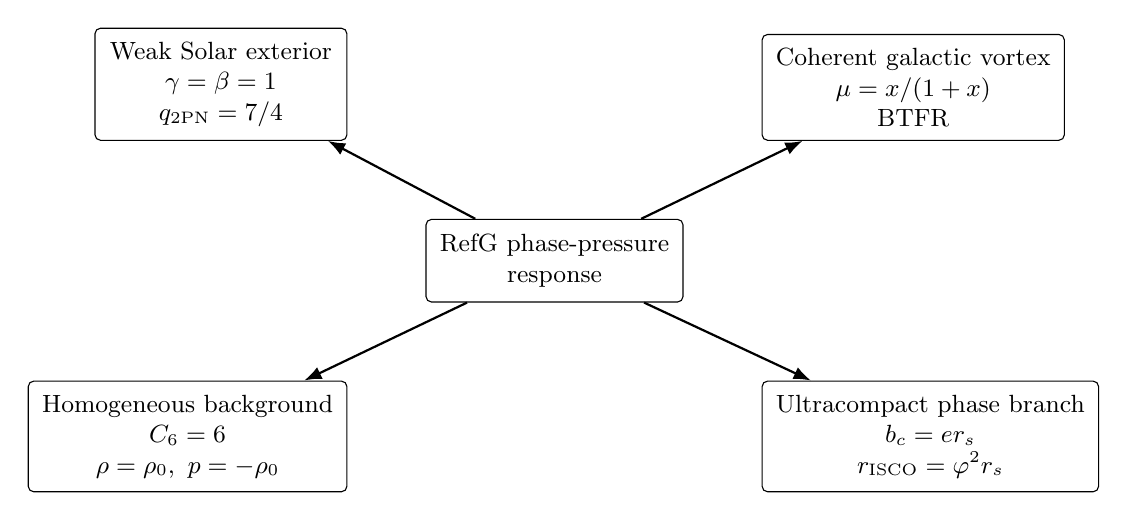
\begin{tikzpicture}[node distance=1.4cm]
\node[regimebox] (core) {RefG phase-pressure\\response};
\node[regimebox, above left=of core] (solar) {Weak Solar exterior\\$\gamma=\beta=1$\\$q_{\rm 2PN}=7/4$};
\node[regimebox, above right=of core] (galaxy) {Coherent galactic vortex\\$\mu=x/(1+x)$\\BTFR};
\node[regimebox, below left=of core] (cosmo) {Homogeneous background\\$C_6=6$\\$\rho=\rho_0,\ p=-\rho_0$};
\node[regimebox, below right=of core] (strong) {Ultracompact phase branch\\$b_c=e r_s$\\$r_{\rm ISCO}=\varphi^2r_s$};

\draw[refgarrow] (core) -- (solar);
\draw[refgarrow] (core) -- (galaxy);
\draw[refgarrow] (core) -- (cosmo);
\draw[refgarrow] (core) -- (strong);
\end{tikzpicture}
\caption{Separation of physical regimes. The same phase-pressure response is read differently in the weak Solar exterior, the coherent galactic vortex, the homogeneous cosmological background, and the ultracompact strong-field phase branch.}
\label{fig:regime-map}
\end{figure}

\section{Tensor Waves}

In the tensor-wave sector one must check whether the introduction of the phase-spatial medium shifts the propagation speed of gravitational waves away from the speed of light.

The standard observational constraint is the event GW170817, according to which a tensor gravitational wave must propagate on the light cone. The minimal phase sector of RefG lies in the subclass of Horndeski theory in which no excess propagation speed of the tensor mode is generated. The formal check therefore begins with this connection.

For the minimal Horndeski class,
\begin{equation}
G_4=\mathrm{const},\qquad G_{4X}=0,\qquad G_5=0 .
\end{equation}
The tensor-speed parameter is
\begin{equation}
\alpha_T=\frac{c_g^2}{c^2}-1 .
\end{equation}
It follows that
\begin{equation}
\alpha_T=0,\qquad c_g=c .
\end{equation}

The tensor-speed check splits into two steps. The first step is the Horndeski/EFT bridge: $G_4=\mathrm{const}$, $G_{4X}=0$, and $G_5=0$ directly give $\alpha_T=0$. The second step is the transverse-traceless (TT) projection of the solid-like sector. In the local Minkowski transverse-traceless sector, the background part of the fields $\phi^A$ creates no additional kinetic-gradient terms of the $\dot h^2$ or $(\partial_z h)^2$ type:
\begin{equation}
\delta K_{\rm TT}=0,\qquad \delta G_{\rm TT}=0 .
\end{equation}
Therefore the TT dispersion is
\begin{equation}
\omega^2=c^2k^2 .
\end{equation}
The solid-like sector leaves the kinetic-gradient speed of the tensor wave unchanged, and in the local TT limit the wave propagates on the light cone:
\begin{equation}
c_g=c .
\end{equation}

The scope of this result is the tensor speed and the local TT dispersion. Additional polarizations, dispersive corrections, and the full waveform phenomenology belong to a separate analysis.

The connection with the galactic MOND channel is read through the separation of regimes. In the galactic regime, the solid-like/vortical response acts as a static, coherent, and anisotropic source. In the gravitational-wave section, the TT projection concerns the transverse-traceless kinetic-gradient speed of the wave. The same medium carries load in a static source while leaving the leading speed of a TT wave unchanged.

Physically, this means that a homogeneous common mode is calibrated together with local standards, while a tensor detector measures the differential shear response. The observable TT-wave signal is therefore compatible with the same framework in which a common background shift is not locally visible.

\section{CMB Test with Identical Input Conditions}

For the cosmic microwave background (CMB), the key test is whether the additional phase-spatial sector of RefG destabilizes the standard results when identical background and perturbative input conditions are used.

The standard formalism in this case is the Einstein--Boltzmann system. It includes the Poisson source, metric slip, gravitational lensing, and the integrated Sachs--Wolfe (ISW) effect. The identical-input test of RefG fixes four conditions: the same $H(a)$, the same matter content, the same recombination history, and the same primordial spectrum.

On this FLRW branch, the Bellini--Sawicki parameters vanish:
\begin{equation}
\alpha_K=\alpha_B=\alpha_M=\alpha_T=0 .
\end{equation}

The Poisson source, metric slip, Weyl potential, CMB lensing source, and ISW source then follow the same linear hierarchy as in LCDM. On the $Z$-extended branch of the $C_6=6$ completion, the identical conditions are fixed by
\begin{align}
\delta C_6 &= 0, \\
\delta Z_{\rm linear} &= 0 .
\end{align}

Under these conditions the linear sources of the completion vanish. The invariant $Z$ is zero on the background; on this branch, its linear source is also zero. The fixed condition on $C_6$ cancels the first variation of the quadratic completion. Therefore, on the branch with identical initial conditions, the linear Einstein--Boltzmann hierarchy of RefG coincides with the LCDM hierarchy:
\begin{equation}
C_\ell^{\rm RefG}=C_\ell^{\rm LCDM}.
\end{equation}

On the same branch, the residuals of the additional source are
\begin{align}
\rho_{\rm RefG}+p_{\rm RefG} &= 0, \\
\delta\rho_{\rm RefG}=\delta p_{\rm RefG} &= 0, \\
q_{\rm RefG} &= 0, \\
\sigma_{\rm RefG} &= 0,
\end{align}
and therefore
\begin{equation}
S_{\rm Poisson}^{\rm extra}
=S_{\rm slip}^{\rm extra}
=S_{\gamma b}^{\rm extra}
=S_{\rm lens}^{\rm extra}
=S_{\rm ISW}^{\rm extra}
=0 .
\end{equation}

Here ``identical input conditions'' means the same background history $H(a)$, the same matter content, the same recombination, and the same primordial spectrum. If the comparison LCDM model contains CDM, it is also included in this identical test. This is the CMB compatibility identity for fixed input conditions; the replacement of particle dark matter is a separate active-Boltzmann problem.

The closed result of this section is the CMB identity for identical input conditions: the additional phase-spatial sector of RefG leaves the standard CMB calculation unchanged when the background history, matter content, recombination, and initial conditions are unchanged. Constructing the CMB without particle dark matter is a separate active-source layer. It requires the source density and velocity, the Euler equation, the closure of the shear response and metric slip, and full comparison with Planck/BAO/lensing data.

\section{Inertia and Mass}

In the inertia sector, the question is what grounds the equivalence between inertial mass and the gravitational source charge.

In the standard formalism, this fact is postulated through the equivalence principle: in free fall, mass cancels out of the equation of motion. In the physical interpretation of RefG, both quantities are equivalent to the same oscillon energy. Inertia is the response of a localized structure to acceleration, while gravitational charge is the long-range refractive source of the same structure.

The formal analysis therefore begins with the Noether four-momentum:
\begin{equation}
P^\mu=\int T^{0\mu}\,d^3x .
\end{equation}
In the rest frame, the localized energy gives
\begin{equation}
P^\mu=\left(\frac{E_0}{c},0,0,0\right).
\end{equation}
After a small Lorentz boost,
\begin{align}
P'^{0} &= \gamma\frac{E_0}{c}, \\
P'^{i} &= \gamma\frac{E_0}{c^2}v^i .
\end{align}
Therefore the momentum is
\begin{equation}
p_i=\gamma\frac{E_0}{c^2}v_i,
\end{equation}
and the low-speed force coefficient is $E_0/c^2$. In RefG, inertia and gravitational charge are tied to the same localized energy. The inertial mass is defined from the Noether four-momentum as
\begin{equation}
M_{\rm inert}=\frac{E_0}{c^2}.
\end{equation}

The zero-frequency asymptotic source fixes the same quantity:
\begin{equation}
M_{\rm source}=\frac{E_0}{c^2}.
\end{equation}

Thus the mass cancels from the equation of free fall. Radiation and delayed effective dressing contributions remain as higher-order corrections to the response; the primary source of the coefficient relating force and acceleration, $F=Ma$, is the zero mode.

For the gravitational core, the sufficient link in the inertia section is the leading Noether channel: localized energy appears as the same coefficient in the inertial response and in the exterior refractive charge. The full microscopic existence of the oscillon, the direct matching of the zero mode, and the complete closure of the Laue integral belong to the particle/structural program. The gravitational core uses this leading energetic identification.

The result connects to the refractive model in the following form: the effective exterior mass is the asymptotic charge of localized oscillon energy that carries the refractive deficit of the base medium. The leading identity between inertial mass and exterior refractive charge is fixed here; the microphysical evolution of the local rest mass belongs to the particle/structural program.

The physical interpretation of inertia is the following. In uniform motion, the localized structure and its exterior refractive profile move in one regime, while acceleration changes this alignment. At leading order, the resistance to this change is tied to the same localized energy that acts as exterior refractive charge.

\section{Strong-Field Branch and Subsequent Layers}
\label{sec:strong-field}

The boundary is drawn as follows. The present paper constructs a self-contained gravitational core, while observational comparison and additional phenomenology move into subsequent layers.

In the leading phase-spherical strong-field branch, the phase potential satisfies the vacuum equation
\begin{equation}
\left(r^2\phi'\right)'=0 .
\end{equation}
The flat limit at infinity and the weak-field normalization fix the solution
\begin{equation}
\phi=-\frac{r_s}{r}.
\end{equation}
The biconformal operational map sends this solution to the exponential exterior
\begin{equation}
ds^2=-\exp\!\left(-\frac{r_s}{r}\right)c^2dt^2
     +\exp\!\left(\frac{r_s}{r}\right)
      \left(dr^2+r^2d\Omega^2\right).
\end{equation}

The exponential-metric class is described in the literature as a traversable-wormhole geometry \cite{Boonserm2018}. In RefG the same static geometry is obtained from the phase strong-field map, and its source is the effective stress $\Theta^{\rm RefG}$. The energy-condition question on this branch is therefore posed for the $\Theta^{\rm RefG}$ source. The geodesic analysis of this exterior gives the photon and massive-orbit markers below.

In this exterior no finite-radius horizon appears. Its strong-field test is therefore directly tied to tests of horizonless ultracompact objects. A full compact-object theory requires the $p01/F_{\rm min}$ source, connection to the inner core, physical energy conditions, a rotating exterior, the QNM/echo channel, and comparison with EHT/ngEHT/BHEX-type ray tracing.

The physical criterion for selecting the branch is the compactness of the source, the exterior matching condition, and the weight of diffuse medium stress in the exterior vacuum. Near an extended weak-field body such as the Sun, stress and radial deformation participate in the 2PN exterior balance and give $q_{\rm 2PN}=7/4$. Near an ultracompact source, the exterior static vacuum is dominated by the phase deficit; therefore $b_c=e r_s$ and $r_{\rm ISCO}=\varphi^2 r_s$ belong to this compact phase branch.

For null rays, the radial barrier is
\begin{equation}
B_{\rm ph}(r)=\frac{\exp(-2r_s/r)}{r^2}.
\end{equation}
Its derivative is proportional to
\begin{equation}
-\frac{2(r-r_s)\exp(-2r_s/r)}{r^4},
\end{equation}
and the photon sphere is therefore located at
\begin{equation}
r_{\rm ph}=r_s .
\end{equation}
At this radius the critical impact parameter is
\begin{equation}
b_c=e r_s .
\end{equation}
Comparison with the static Schwarzschild value in GR,
\begin{equation}
b_c^{\rm GR}=\frac{3\sqrt3}{2}r_s,
\end{equation}
gives a $+4.63\%$ scale shift of the shadow.

For a massive test body, the effective potential is
\begin{equation}
V_{\rm eff}=\exp\!\left(-\frac{r_s}{r}\right)
 +\frac{L^2}{r^2}\exp\!\left(-\frac{2r_s}{r}\right).
\end{equation}
The circular-orbit condition $dV_{\rm eff}/dr=0$ gives
\begin{equation}
L_{\rm circ}^2
=\frac{r^2r_s\exp(r_s/r)}{2(r-r_s)}.
\end{equation}
Massive circular orbits therefore begin outside the photon boundary, $r>r_s$. The marginal-stability condition $d^2V_{\rm eff}/dr^2=0$ reduces the problem to one polynomial:
\begin{equation}
r^2-3r_sr+r_s^2=0 .
\end{equation}
The physical root is
\begin{equation}
r_{\rm ISCO}
=\frac{3+\sqrt5}{2}r_s
=\varphi^2r_s .
\end{equation}
The same geodesic chain gives the ISCO frequency ratio for the same mass. In the exponential branch,
\begin{equation}
\Omega^2=
\frac{c^2r_s\exp(-2r_s/r)}
{r^2(2r-r_s)} ,
\end{equation}
while the Schwarzschild reference value is
\begin{equation}
\Omega_{\rm GR}^2=\frac{c^2}{54r_s^2}.
\end{equation}
Substitution of $r_{\rm ISCO}=\varphi^2r_s$ gives
\begin{equation}
f_{\rm ISCO}=0.931\,f_{\rm ISCO}^{\rm GR}.
\end{equation}

\begin{figure}[t]
\centering
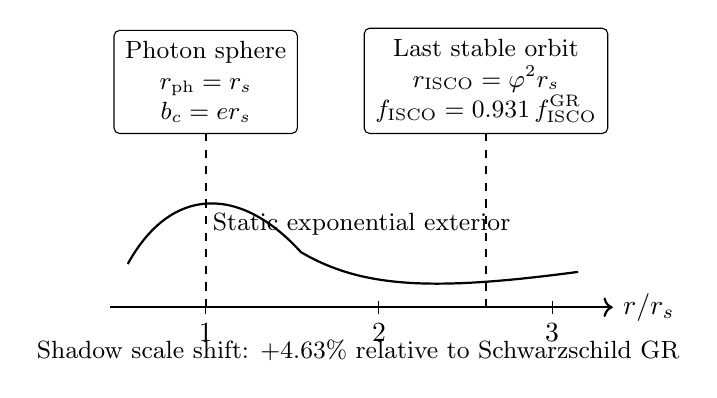
\begin{tikzpicture}[x=2.2cm,y=1cm]
\draw[->, thick] (0.45,0) -- (3.35,0) node[right] {$r/r_s$};
\foreach \x/\lab in {1/$1$,2/$2$,3/$3$}
  \draw (\x,0.08) -- (\x,-0.08) node[below] {\lab};

\draw[dashed, thick] (1,0) -- (1,2.2);
\node[markerbox, above] at (1,2.2) {Photon sphere\\$r_{\rm ph}=r_s$\\$b_c=e r_s$};

\draw[dashed, thick] (2.618,0) -- (2.618,2.2);
\node[markerbox, above] at (2.618,2.2) {Last stable orbit\\$r_{\rm ISCO}=\varphi^2r_s$\\$f_{\rm ISCO}=0.931\,f_{\rm ISCO}^{\rm GR}$};

\draw[thick] (0.55,0.55) .. controls (0.8,1.55) and (1.2,1.55) .. (1.55,0.7)
             .. controls (1.9,0.25) and (2.3,0.2) .. (3.15,0.45);
\node[align=center,font=\small] at (1.9,1.05) {Static exponential exterior};
\node[align=center,font=\small] at (1.88,-0.55) {Shadow scale shift: $+4.63\%$ relative to Schwarzschild GR};
\end{tikzpicture}
\caption{Static strong-field markers of the phase-spherical exponential branch. The photon barrier fixes $r_{\rm ph}=r_s$ and $b_c=e r_s$; marginal stability of massive circular orbits fixes $r_{\rm ISCO}=\varphi^2r_s$.}
\label{fig:strong-field-markers}
\end{figure}

Thus the static branch fixes the photon barrier, the shadow scale, and the golden-ratio ISCO in one picture. No additional free parameter is used in this chain.

The status of this result is clear. The static spherical phase branch is closed at the level of the phase equation, the biconformal map, and geodesic analysis. The full $RefG/F_{\rm min}$ compact solution requires the $p01/F_{\rm min}$ stress source, connection to the compact source, and completion of the nonlinear strong-field terms.

The observational test of this static result moves to a rotating exterior, accretion and plasma models, ray tracing, QNM/echo analysis, and comparison with EHT/ngEHT/BHEX data. Here the strong-field sector enters as the static spherical result obtained from the phase equation and as the starting point of the subsequent observational program.

The particle sector belongs to an independent research program, in which the oscillon structure, charge, spin, mass spectrum, and the bridge to the Standard Model are formulated by a strict mathematical formalism. Experimental signatures of the N4/X17 type also belong to this particle and laboratory program. The conclusions of the gravitational core stand on the chain of the action, active stress, refractive source, weak-field limit, and static strong-field marker.

\section{Falsification Criteria}

The physical consistency of RefG is tested by several independent criteria. Local stability, Solar-System 1PN/2PN compatibility, $c_g=c$ in the tensor sector, and the CMB test with identical input conditions are required compatibility conditions. The central falsifiable marker of the paper lies on the static strong-field phase branch: $b_c=e r_s$, a $+4.63\%$ shadow-scale shift relative to the Schwarzschild value in GR, $r_{\rm ISCO}=\varphi^2r_s$, and $f_{\rm ISCO}=0.931\,f_{\rm ISCO}^{\rm GR}$.

Observational separation of this marker requires percent-level shadow-scale accuracy, a rotating compact-source model, accretion/plasma control, and EHT/ngEHT/BHEX-class ray-tracing comparison. Cosmological dynamics, MOND/clusters, and the CMB without particle dark matter remain separate data-test channels.

The detailed observational status is summarized in the following table.

\section{Observational Summary}

\begin{table}[htbp]
\centering
\caption{Summary of sectors, results, and subsequent tests}
\label{tab:observational-summary}
\scriptsize
\setlength{\tabcolsep}{3pt}
\begin{tabularx}{\textwidth}{@{}>{\raggedright\arraybackslash}p{0.13\textwidth}>{\raggedright\arraybackslash}p{0.16\textwidth}XX@{}}
\toprule
Sector & Scope & Result obtained & Subsequent test \\
\midrule
Action & Minimal core &
Minimal Einstein--Hilbert (EH) plus phase/solid-like effective field theory (EFT) core. &
Full EFT basis and higher-order operators. \\

Refractive source & Weak static limit &
Active stress enters the Bianchi/TOV source; the differential chain $\Pi_B'\to h_{\rm eff}\to n_{\rm eff}$ gives the Newtonian Bernoulli channel. &
Full nonspherical field equations. \\

MOND & Spherical vortical limit &
The phase-cycle normalization fixes $a_0=cH_0/(2\pi)$; within the two-channel vortical construction one obtains $\mu=x/(1+x)$ and the BTFR. &
RefG-dynamical vortical derivation, $2\pi$ normalization, SPARC/RAR data, disk curl corrections, and comparison with galaxy-cluster maps. \\

Stability & Local window &
On a homogeneous background there exists a short-wave local window satisfying the no-ghost and principal-symbol conditions. &
Global hyperbolicity, curved backgrounds, and the full Lorentzian perturbation sector. \\

Cosmology & Background balance &
$C_6=6$ gives an exact background $\Lambda$CDM-type algebraic balance; the redshift channel requires compatibility with the CMB blackbody spectrum, SNe $(1+z)$ time dilation, and the Tolman $(1+z)^4$ surface-brightness law. &
Attractor dynamics, $H(z)$, $w(z)$, and comparison with BBN/CMB/BAO/SNe data. \\
\bottomrule
\end{tabularx}
\end{table}

\begin{table}[htbp]
\centering
\caption{Summary of sectors, results, and subsequent tests, continued}
\scriptsize
\setlength{\tabcolsep}{3pt}
\begin{tabularx}{\textwidth}{@{}>{\raggedright\arraybackslash}p{0.13\textwidth}>{\raggedright\arraybackslash}p{0.16\textwidth}XX@{}}
\toprule
Sector & Scope & Result obtained & Subsequent test \\
\midrule
Solar System & Weak physical Solar exterior &
The physical weak Solar exterior has $\gamma=\beta=1$, $\alpha_i=0$, $q_{\rm 2PN}=7/4$; the values $q_{\rm 2PN}=10$, $11/4$, and $2$ belong to other regimes. &
Finite-core connection, final PPN form, and ephemeris comparison. \\

Gravitational waves (GW) & Tensor sector &
$\alpha_T=0$, $c_g=c$. &
Additional polarizations and full waveforms. \\

Cosmic microwave background (CMB) & Compatibility test &
On the branch with fixed identical input conditions, the additional linear sources vanish and $C_\ell^{\rm RefG}=C_\ell^{\rm LCDM}$. &
Active Boltzmann branch without particle dark matter and comparison with Planck/BAO/lensing data. \\

Inertia & Leading Noether channel &
Inertial mass and exterior refractive charge are tied to the same localized energy. &
Direct zero-mode connection, Laue integral, and full oscillon microphysics. \\

Strong field & Leading phase-spherical exponential branch &
$r_{\rm ph}=r_s$, $b_c=e r_s$, $r_{\rm ISCO}=\varphi^2r_s$, $f_{\rm ISCO}=0.931\,f_{\rm ISCO}^{\rm GR}$; the static shadow scale shifts by $+4.63\%$ relative to the Schwarzschild GR value. &
$p01/F_{\rm min}$ compact-source solution, nonlinear strong-field terms, rotating exterior, ray tracing, accretion/plasma model, QNM/echo, and EHT/ngEHT/BHEX comparison. \\

Particles & Boundary layer &
An independent research program; the gravitational argument stands on the chain of action, active stress, and refractive source. &
Development of the full oscillon, gauge, and radiative theoretical program. \\
\bottomrule
\end{tabularx}
\end{table}

\section{Conclusions}

RefG is a phase-spatial framework of effective field theory (EFT) in which the source of gravity is interpreted as a refractive deficit of the base medium. The weak-field Solar-System branch is compatible with GR, while the difference lies in the mechanism itself: Newtonian force, the spherical MOND limit, inertial charge, and the cosmological background balance are written in the language of one phase-pressure response.

The central line of the paper is the following. The minimal action and the active-stress convention lead to the weak static refractive source-index chain; this chain is compatible with the local stability window, the Solar-System 1PN/2PN limit, the tensor result $c_g=c$, the CMB test with identical initial conditions, and the Noether channel of inertia.

The static strong-field axis stands on the leading phase-spherical branch, where the phase equation and the biconformal map give an exponential exterior. On this exterior the photon barrier gives $b_c=e r_s$, while the marginal stability of massive orbits gives $r_{\rm ISCO}=\varphi^2r_s$ and $f_{\rm ISCO}=0.931\,f_{\rm ISCO}^{\rm GR}$. The static shadow scale changes by $+4.63\%$ relative to the Schwarzschild GR value. The full compact-source closure moves to the $p01/F_{\rm min}$ stress, source connection, and rotating strong-field work. The Solar-System result $q_{\rm 2PN}=7/4$ remains in the weak physical exterior branch; the strong-field phase value $q_{\rm 2PN}=2$ is a separate strong-field branch.

\section{Funding}

The study was carried out independently.

\section{Conflict of Interest}

The author declares no conflict of interest.

\begin{thebibliography}{38}

\bibitem{Horndeski1974}
G. W. Horndeski, ``Second-order scalar-tensor field equations in a four-dimensional space,'' \textit{International Journal of Theoretical Physics} \textbf{10}, 363--384 (1974).

\bibitem{Gubitosi2013}
G. Gubitosi, F. Piazza, and F. Vernizzi, ``The effective field theory of dark energy,'' \textit{JCAP} \textbf{02}, 032 (2013).

\bibitem{BelliniSawicki2014}
E. Bellini and I. Sawicki, ``Maximal freedom at minimum cost: linear large-scale structure in general modifications of gravity,'' \textit{JCAP} \textbf{07}, 050 (2014).

\bibitem{AbbottGW170817}
B. P. Abbott et al., ``GW170817: Observation of gravitational waves from a binary neutron star inspiral,'' \textit{Physical Review Letters} \textbf{119}, 161101 (2017).

\bibitem{AbbottGRB170817A}
B. P. Abbott et al., ``Gravitational waves and gamma-rays from a binary neutron star merger: GW170817 and GRB 170817A,'' \textit{Astrophysical Journal Letters} \textbf{848}, L13 (2017).

\bibitem{Endlich2013}
S. Endlich, A. Nicolis, and J. Wang, ``Solid inflation,'' \textit{JCAP} \textbf{10}, 011 (2013).

\bibitem{Nicolis2015}
A. Nicolis, R. Penco, F. Piazza, and R. Rattazzi, ``Zoology of condensed matter: framids, ordinary stuff, extra-ordinary stuff,'' \textit{JHEP} \textbf{06}, 155 (2015).

\bibitem{Milgrom1983}
M. Milgrom, ``A modification of the Newtonian dynamics as a possible alternative to the hidden mass hypothesis,'' \textit{Astrophysical Journal} \textbf{270}, 365--370 (1983).

\bibitem{Bekenstein2004}
J. D. Bekenstein, ``Relativistic gravitation theory for the modified Newtonian dynamics paradigm,'' \textit{Physical Review D} \textbf{70}, 083509 (2004).

\bibitem{Verlinde2017}
E. P. Verlinde, ``Emergent gravity and the dark universe,'' \textit{SciPost Physics} \textbf{2}, 016 (2017).

\bibitem{ChamseddineMukhanov2013}
A. H. Chamseddine and V. Mukhanov, ``Mimetic dark matter,'' \textit{Journal of High Energy Physics} \textbf{11}, 135 (2013).

\bibitem{Lelli2016}
F. Lelli, S. S. McGaugh, and J. M. Schombert, ``SPARC: Mass models for 175 disk galaxies with Spitzer photometry and accurate rotation curves,'' \textit{Astronomical Journal} \textbf{152}, 157 (2016).

\bibitem{McGaugh2016}
S. S. McGaugh, F. Lelli, and J. M. Schombert, ``Radial acceleration relation in rotationally supported galaxies,'' \textit{Physical Review Letters} \textbf{117}, 201101 (2016).

\bibitem{Clowe2006}
D. Clowe, M. Bradac, A. H. Gonzalez, M. Markevitch, S. W. Randall, C. Jones, and D. Zaritsky, ``A direct empirical proof of the existence of dark matter,'' \textit{Astrophysical Journal Letters} \textbf{648}, L109--L113 (2006).

\bibitem{Will1993}
C. M. Will, \textit{Theory and Experiment in Gravitational Physics}, Cambridge University Press (1993).

\bibitem{Will2014}
C. M. Will, ``The confrontation between general relativity and experiment,'' \textit{Living Reviews in Relativity} \textbf{17}, 4 (2014).

\bibitem{MaBertschinger1995}
C.-P. Ma and E. Bertschinger, ``Cosmological perturbation theory in the synchronous and conformal Newtonian gauges,'' \textit{Astrophysical Journal} \textbf{455}, 7 (1995).

\bibitem{Lewis2000}
A. Lewis, A. Challinor, and A. Lasenby, ``Efficient computation of CMB anisotropies in closed FRW models,'' \textit{Astrophysical Journal} \textbf{538}, 473--476 (2000).

\bibitem{Blas2011}
D. Blas, J. Lesgourgues, and T. Tram, ``The Cosmic Linear Anisotropy Solving System (CLASS). Part II: Approximation schemes,'' \textit{JCAP} \textbf{07}, 034 (2011).

\bibitem{Planck2018}
Planck Collaboration, ``Planck 2018 results. VI. Cosmological parameters,'' \textit{Astronomy \& Astrophysics} \textbf{641}, A6 (2020).

\bibitem{Bertotti2003}
B. Bertotti, L. Iess, and P. Tortora, ``A test of general relativity using radio links with the Cassini spacecraft,'' \textit{Nature} \textbf{425}, 374--376 (2003).

\bibitem{Creminelli2017}
P. Creminelli and F. Vernizzi, ``Dark energy after GW170817 and GRB170817A,'' \textit{Physical Review Letters} \textbf{119}, 251302 (2017).

\bibitem{SaksteinJain2017}
J. Sakstein and B. Jain, ``Implications of the neutron star merger GW170817 for cosmological scalar-tensor theories,'' \textit{Physical Review Letters} \textbf{119}, 251303 (2017).

\bibitem{Deffayet2009}
C. Deffayet, G. Esposito-Farese, and A. Vikman, ``Covariant Galileon,'' \textit{Physical Review D} \textbf{79}, 084003 (2009).

\bibitem{Kobayashi2011}
T. Kobayashi, M. Yamaguchi, and J. Yokoyama, ``Generalized G-inflation: inflation with the most general second-order field equations,'' \textit{Progress of Theoretical Physics} \textbf{126}, 511--529 (2011).

\bibitem{Gleyzes2015}
J. Gleyzes, D. Langlois, F. Piazza, and F. Vernizzi, ``Exploring gravitational theories beyond Horndeski,'' \textit{JCAP} \textbf{02}, 018 (2015).

\bibitem{LangloisNoui2016}
D. Langlois and K. Noui, ``Degenerate higher derivative theories beyond Horndeski: evading the Ostrogradski instability,'' \textit{JCAP} \textbf{02}, 034 (2016).

\bibitem{BenAchour2016}
J. Ben Achour, D. Langlois, and K. Noui, ``Degenerate higher order scalar-tensor theories beyond Horndeski and disformal transformations,'' \textit{Physical Review D} \textbf{93}, 124005 (2016).

\bibitem{Crisostomi2016}
M. Crisostomi, K. Koyama, and G. Tasinato, ``Extended scalar-tensor theories of gravity,'' \textit{JCAP} \textbf{04}, 044 (2016).

\bibitem{Cheung2008}
C. Cheung, P. Creminelli, A. L. Fitzpatrick, J. Kaplan, and L. Senatore, ``The effective field theory of inflation,'' \textit{JHEP} \textbf{03}, 014 (2008).

\bibitem{Endlich2014}
S. Endlich, B. Horn, A. Nicolis, and J. Wang, ``Squeezed limit of the solid inflation three-point function,'' \textit{Physical Review D} \textbf{90}, 063506 (2014).

\bibitem{Bordin2017}
L. Bordin, P. Creminelli, M. Mirbabayi, and J. Norena, ``Solid consistency,'' \textit{JCAP} \textbf{03}, 004 (2017).

\bibitem{Kostelecky2011}
V. A. Kostelecky and N. Russell, ``Data tables for Lorentz and CPT violation,'' \textit{Reviews of Modern Physics} \textbf{83}, 11--31 (2011).

\bibitem{WillNordtvedt1972}
C. M. Will and K. Nordtvedt Jr., ``Conservation laws and preferred frames in relativistic gravity. I. Preferred-frame theories and an extended PPN formalism,'' \textit{Astrophysical Journal} \textbf{177}, 757--774 (1972).

\bibitem{Damour1992}
T. Damour and G. Esposito-Farese, ``Tensor-multi-scalar theories of gravitation,'' \textit{Classical and Quantum Gravity} \textbf{9}, 2093--2176 (1992).

\bibitem{Damour1993}
T. Damour and G. Esposito-Farese, ``Nonperturbative strong-field effects in tensor-scalar theories of gravitation,'' \textit{Physical Review Letters} \textbf{70}, 2220--2223 (1993).

\bibitem{Damour1996}
T. Damour and G. Esposito-Farese, ``Tensor-scalar gravity and binary-pulsar experiments,'' \textit{Physical Review D} \textbf{54}, 1474--1491 (1996).

\bibitem{Boonserm2018}
P. Boonserm, T. Ngampitipan, A. Simpson, and M. Visser, ``Exponential metric represents a traversable wormhole,'' \textit{Physical Review D} \textbf{98}, 084048 (2018).

\end{thebibliography}

\end{document}
